\newpage
\subsection{Wellen}
\textbf{Doppelpendel}\\
\begin{minipage}{0.69\textwidth}
Betrachte zwei Kugeln, welche mit Federn verbunden sind (vgl. Abbildung). Die Kugeln
haben beide die Masse m, die Federn haben alle die Federkonstante k, und die ungespannten Längen sind $l = L /3$.
\[
	\begin{array}{l}
		m \ddot{y}_1 = -k(y_1-l) +mg + k(y_2-l-y_1)\\
		m \ddot{y}_2 = -k(y_2-l) +mg + k(y_2-l-y_1)\\
		\textrm{ Durch Addition ergibt sich}\\
		m(\ddot{y}_1 + \ddot{y}_2) = -k (y_1+y_2) +2mg +3kl\\
		\textrm{Definition der Schwerpunktskoordinaten } \;y_s = \frac{y_1 + y_2}{2}\\
		m(\ddot{y}_1 + \ddot{y}_2) = -k y_s +mg +\frac{3}{2} kl \Rightarrow \ddot{y}_s + \frac{k}{s} y_s = g +\frac{3}{2} \frac{kl}{m} \\
		y(s) = A_s\cdot \sin (\omega_s t+\varphi_s) +\frac{mg}{k} + \frac{3}{2} l  \qquad \omega_s = \sqrt{\frac{k}{m}}
		\textrm{ Durch Subtraktion ergibt sich:}\\
		m(\ddot{y}_1 -\ddot{y}_2 +3k(y_1 -y_2) = -3kl\\
		\textrm{Definition der Relativbewegung }\; y_d = y_1-y_2\\
		\ddot{y}_d +\frac{3k}{m}y_d =\frac{-3kl}{m}\\
		y_d =  A_D\cdot \sin(\omega_d t+\varphi_d) -l \quad \omega_d = \sqrt{\frac{3k}{m}}\\
		y_1(t) = y_s+\frac{y_d}{2} \qquad y_2 = y_s - \frac{y_d}{2}
	\end{array}
\]
\end{minipage}
\hfill
\begin{minipage}{0.29\textwidth}
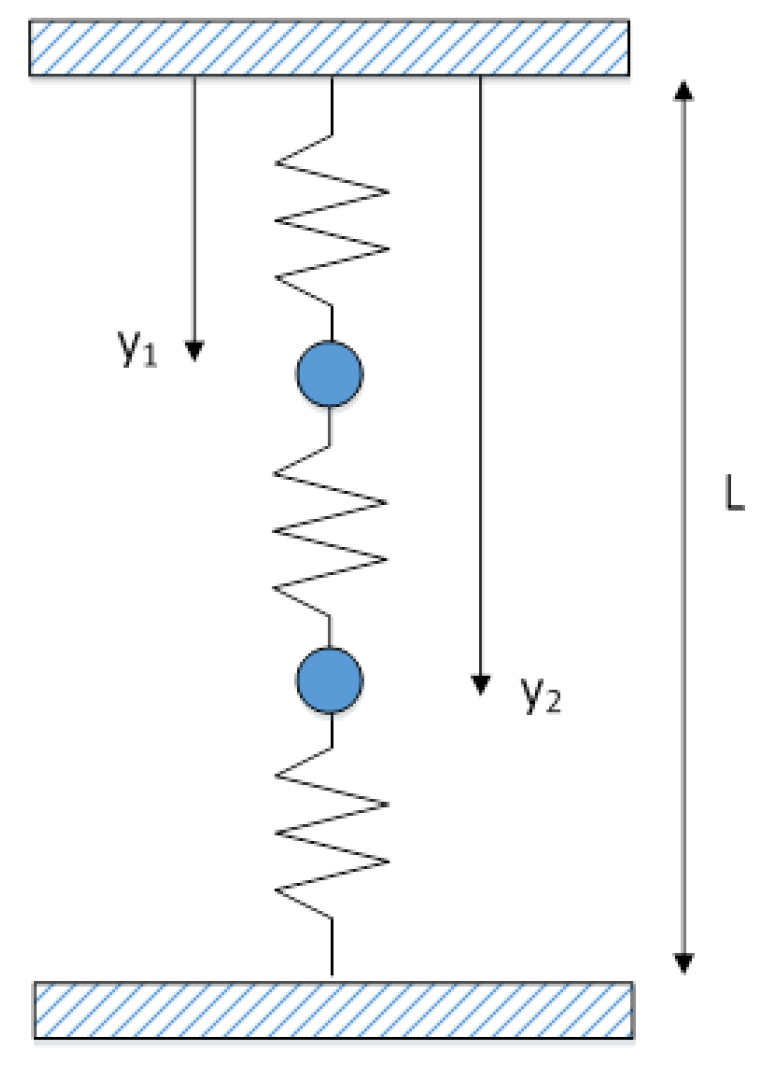
\includegraphics[width = 0.8\textwidth]{bilder/a91.png}
\end{minipage}





\textbf{Longitudinale Welle in Metallstab}\\
Ausbreitung der Geschwindigkeit einer Welle in einem Metallstab. (Der Stab wird auf die Kopfseite geschlagen, Longitudinale Welle).
\begin{align*}
E_{Stahl} &= 210GPa = \textrm{Elastitzizätsmodul}\\
\varrho_{Stahl} &= 7850 \frac{kg}{m^3}
m = \varrho A h \\
c &= E \frac{A}{h}\\
u^2 &= \frac{ch^2}{m} = \frac{(\frac{EA}{h})h^2}{\varrho A h} = \frac{E}{\varrho}  \Rightarrow u = \sqrt{\frac{E}{\varrho}} =\frac{2.1\cdot 10^11 Pa}{7850 \frac{kg}{m^3}} = 5172\frac{m}{s}
\end{align*}
\textbf{Schwingung einer Saite} (stehende Welle)\\
Eine Stahlseite der Länge $l=0.5m$. Die Saite ist fest eingespannt mit einer Zugkraft $F= 100N$ und einem Durchmesser $d=1mm$. Die Dichte der Stahlsaite ist $\varrho = 7850\frac{kg}{m^3}$
\begin{align*}
u&=2\cdot f \Rightarrow f = \frac{u}{2}\\
u&= \sqrt{\frac{F}{\varrho\cdot A}}\\
\lambda_1&= 2\cdot l = 2m\\
\lambda_n &= \frac{2\cdot L}{n}\\
A &= \pi\frac{D^2}{4} = \pi \frac{(10^{-3})^2}{4} = 7.85\cdot 10^{-7}m^2\\
u&= \sqrt{\frac{100N}{7850\cdot 7.85\cdot 10^{-7}}}=127.12 Hz
\end{align*}

\textbf{Stehende Welle in einem Rohr} (Bierflaschengrundton)

Ein Rohr mit einem offenen Ende (Bsp. Bierflasche) hat den Grundton $A = 440Hz$ Wie lang ist das Rohr bei $T = 293K$? Wie müsste man die Temperatur im Rohr ändern um eine Frequenz von $415.3Hz$ zu erzeugen.\\
\begin{align*}
L&=\frac{\lambda}{4} + n\frac{\lambda}{2}\quad \kappa= 1.4  \quad M=28.8\cdot 10^{-3}\frac{kg}{mol} \quad R=8.314\frac{J}{mol\cdot K}\\
u&=\sqrt{\frac{\kappa\cdot R\cdot T}{M}}=\sqrt{\frac{1.4\cdot 8.314\cdot 293}{29}}
\end{align*}

\textbf{Schwebung mit Klaviersaite}\\
$f_1 = 600Hz$, $f_2 = 606Hz$, $\Delta f = 6Hz$
\begin{align*}
u&=\sqrt{\frac{F}{\varrho\cdot A}}\\
f&=\frac{u}{2}\\
\lambda &= 2\cdot L\\
f_1&=\frac{1}{\lambda}\sqrt{\frac{F_1}{\varrho\cdot A}}\\
\frac{f_1}{f_2} &= \sqrt{\frac{F_1}{F_2}}\Rightarrow \frac{F_2}{F_1} = \left(\frac{f_2}{f_1}\right)^2 = \left(\frac{606Hz}{600Hz}\right)^2 = \frac{1.0201}{1}
\end{align*}



\textbf{Dopplereffekt}
\textbf{Frequenzvergleich}\\
Ein Auto fährt hupend mit einer Geschwindigkeit von 111 km/h dicht an einem ruhenden Beobachter vorbei. Um wieviel ändert sich die Tonhöhe? Die Lufttemperatur beträgt $\vartheta = 14.3^\circ C$, die mittlere Molmasse der Luft: $M=0.02883 g/mol$, der Adiabatenexponent der Luft: $\kappa = 1.4$\\
\begin{align*}
u&= \sqrt{\frac{\kappa R T}{M}} = \sqrt{\frac{1.4\cdot 8.3145\cdot (273.15+14.3)K}{0.02883}} = 340.676m/s\\
f_1 &= \frac{1}{1-\frac{v}{u}}\cdot f\\
f_2 &= \frac{1}{1+\frac{v}{u}}\cdot f\\
\frac{f_1}{f_2} &= \frac{\frac{1}{1-\frac{v}{u}}}{\frac{1}{1+\frac{v}{u}}} = \frac{\frac{1}{1-\frac{111/3.6}{340.676}}}{\frac{1}{1+\frac{111/3.6}{340.676}}} = 1.199
\end{align*}
\textbf{Bewegte Quelle und bewegter Beobachter}\\
Auf einer Strasse, die dicht an einer Bahnlinie entlang führt, fährt ein Motorradfahrer mit einer Geschwindigkeit $v_B =  90 km/h$. Ein Zug kommt ihm mit $v_Q =  120 km/h$ entgegen. Die Lokomotive pfeift mit einer Frequenz $f_q$ von 1000 Hz. Welche Frequenz hat der Ton, den
der Motorradfahrer hört? Die Schallgeschwindigkeit beträgt 343 m/s.
\[
f_B = \frac{u+v_B \cos(\vartheta_B)}{u-v_Q \cdot \cos(\vartheta_Q)}\cdot f_q = \frac{343+(90/3.6)m/s}{343-(120/3.6)m/s} \cdot 1kHz = 1188.4Hz
\]


\begin{minipage}{0.59\textwidth}
\textbf{Machscher Kegel}\\
Ein Geschoss fliegt mit der Geschwindigkeit $v = 660 m/s$ in einem Abstand $a=5m$ an einem Mann vorbei. Wie weit ist das Geschoss vom Mann entfernt, wenn er es hört? Schallgeschwindigkeit $u = 329.6m/s$
\begin{align*}
\sin(\vartheta) &= \frac{u}{v} = \frac{a}{d}\\
d&=\frac{v\cdot a}{u} = \frac{660\cdot 5}{329.6} = 10.01\frac{m}{s}
\end{align*}
\end{minipage}
\begin{minipage}{0.4\textwidth}
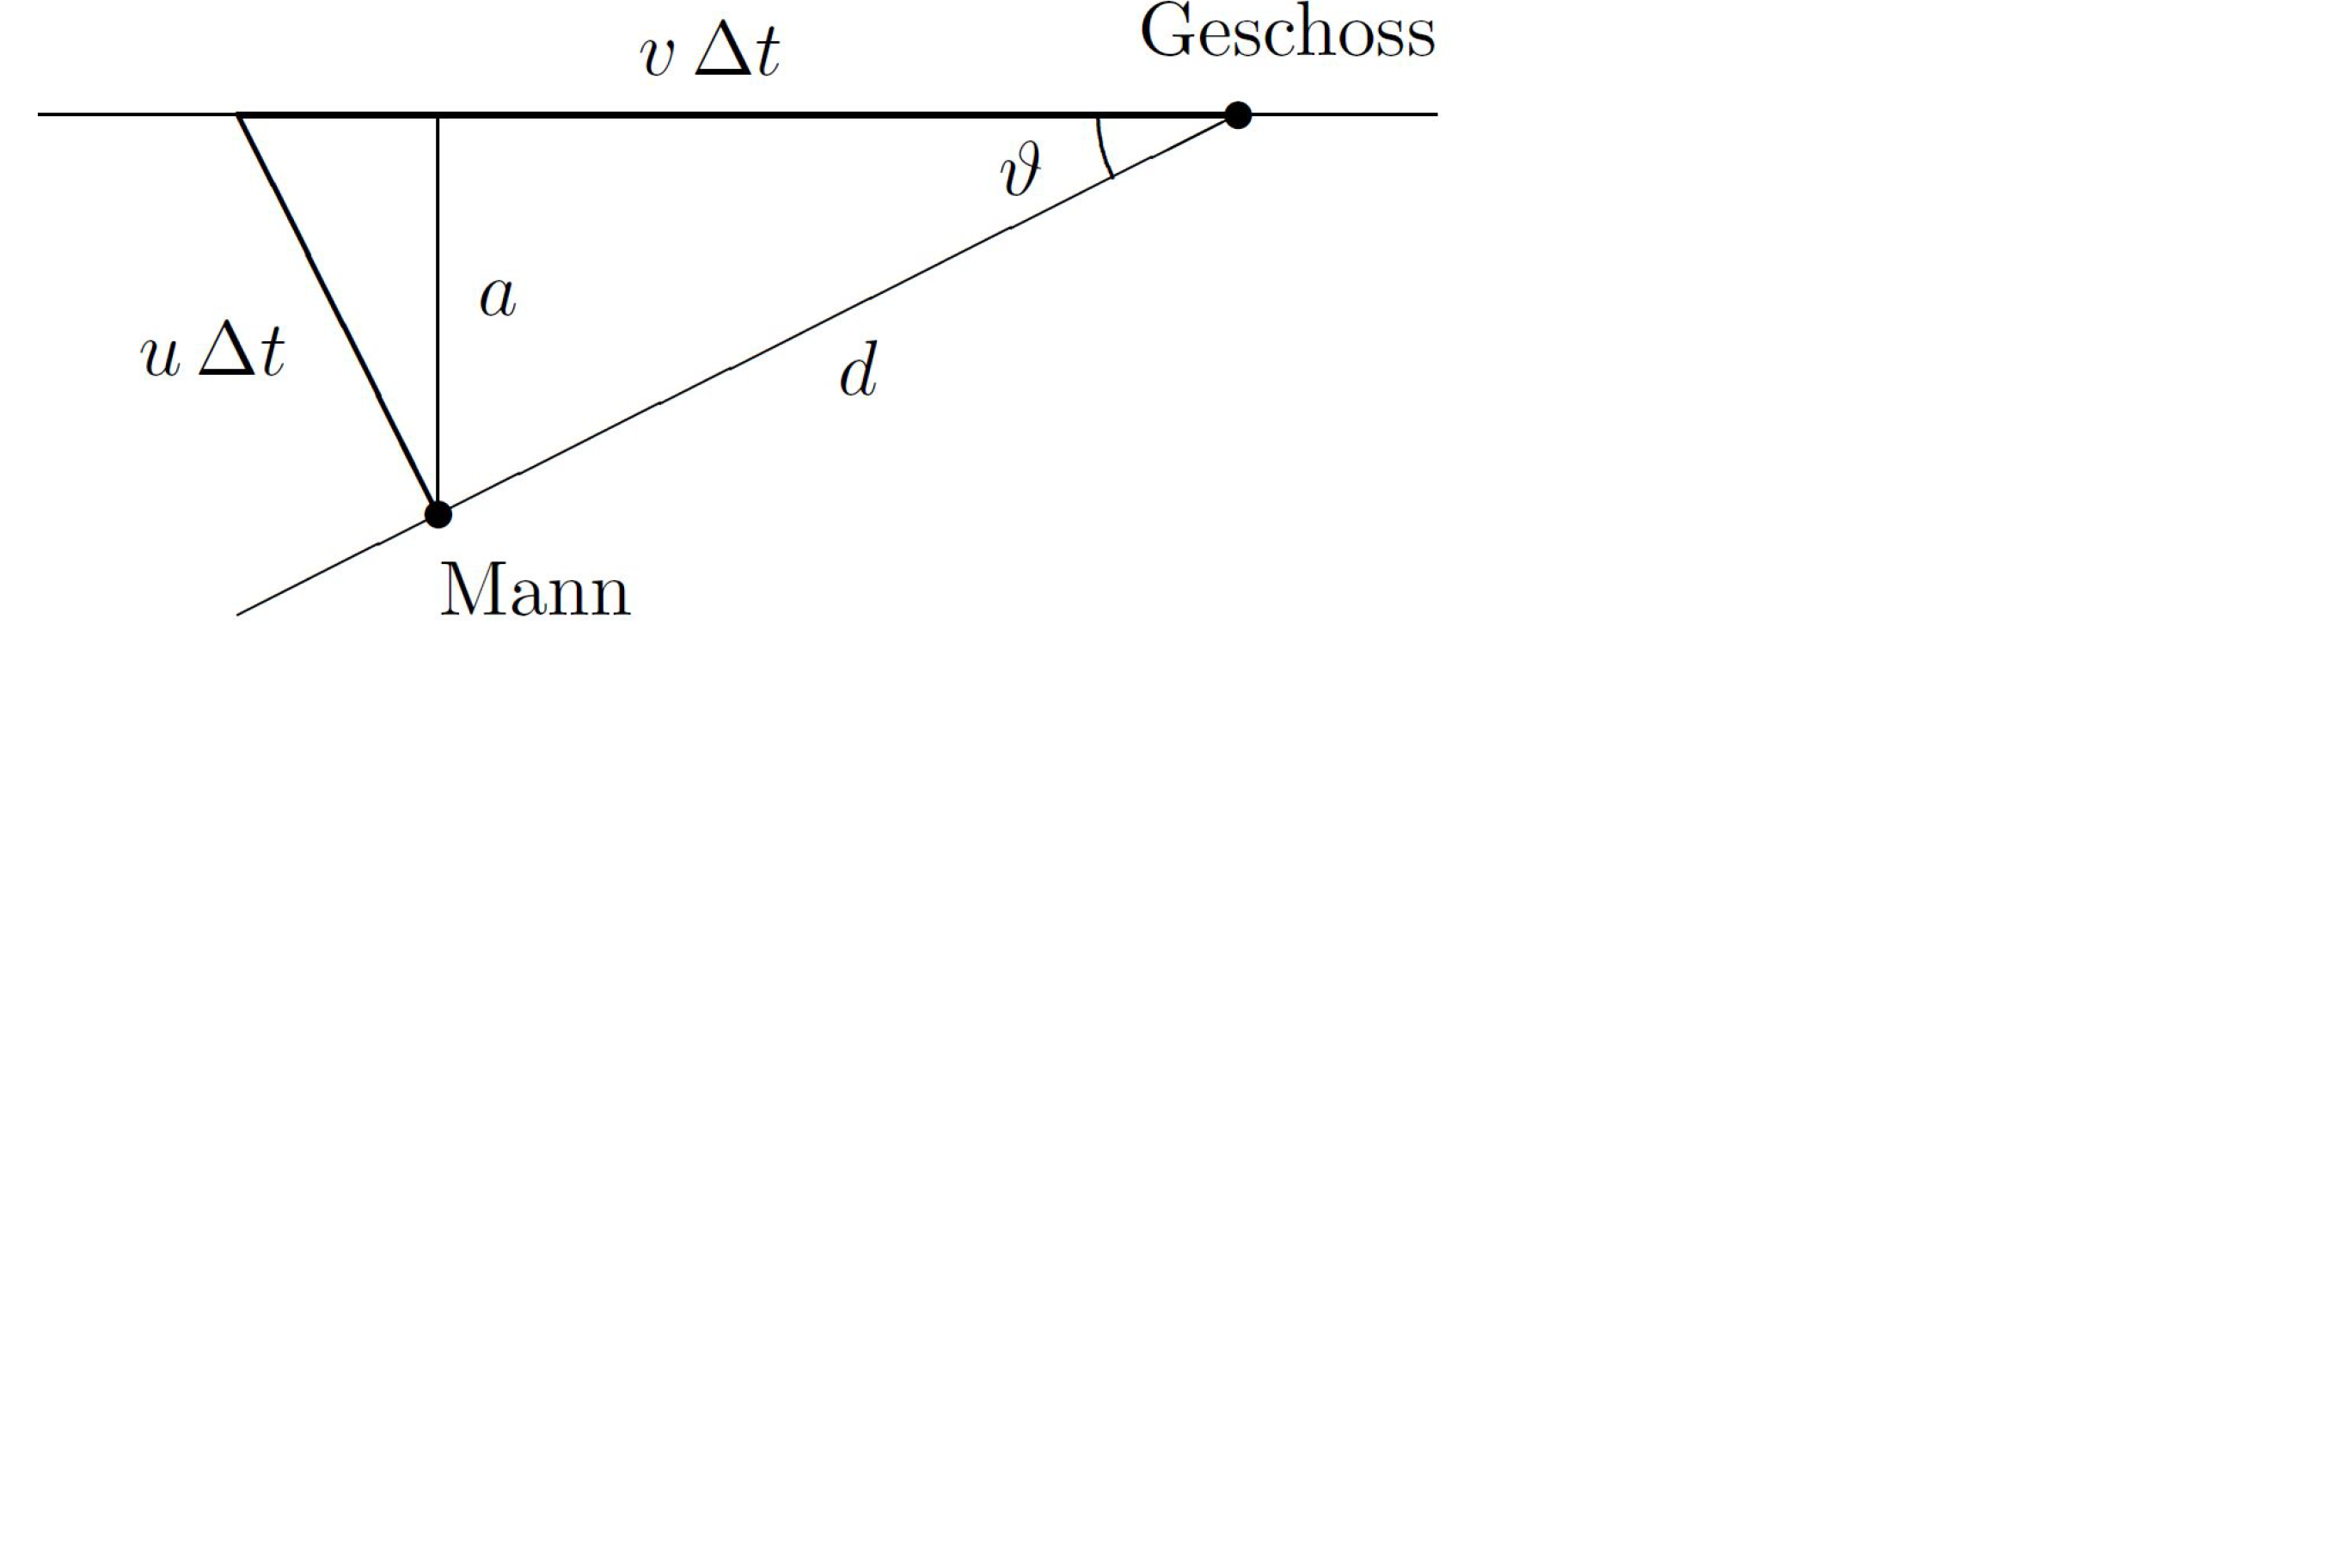
\includegraphics[width = 0.99\textwidth]{bilder/a113.png}
\end{minipage}

\textbf{Radarfalle}
Einem Auto wird von hinten unter einem Winkel $\vartheta = 160^\circ$ zur Fahrtrichtung ein Radarsignal mit der Frequenz $f_s = 1.8 GHz$ nachgesandt. Das reflektierte Signal wird mit der Senderfrequenz
 überlagert und erzeugt eine Schwebungsfrequenz $f_{\textrm{schweb}}  = 240 Hz$. Wie schnell fährt das Auto?\\

Aus der Formel $f' = \frac{\sqrt{1-\beta^2}}{1-\beta \cos(\vartheta)}\cdot f_s$ mit $\beta = \frac{v}{c}$ und mit $c= $ Lichtgeschwindigkeit $= 299'792'458 m/s$ lässt sich für Verhältnismässig kleine $v$ folgende Gleichung herleiten
\[
	\beta =\frac{v}{c} = \frac{-v_{\textrm{schweb}}}{2\cos(\beta)\cdot f_s} \Rightarrow v= \frac{-v_{\textrm{schweb}}\cdot c}{2\cos(\beta)} = \frac{-240\cdot 299'762'458}{2\cos(160)} = 21.267m/s = 76.56km/h
\]

\newpage

\textbf{Beispiel Interferenz mit Schallwellen}\\
Zwei Schallquellen schwingen in Phase mit der Amplitude $p_0$. An einem Punkt der sich $s_1 = 5m$ von der ersten Quelle und $s_2 = 5.17m$ von der zweiten Quelle entfernt befindet ist die Amplitude der Welle zu bestimmen die Frequenz $f = 500 Hz$ die Schallgeschwindigkeit $u= 340m/s$

\begin{minipage}{0.6\textwidth}
\begin{align*}
	\Delta x &= s_1-s_2 = 0.17m\\
	\lambda&= \frac{u}{f} = \frac{340m/s}{500} = 0.68m = 4\cdot \Delta x\\
	\delta &= \frac{2\pi\cdot \Delta x}{\lambda} = \frac{\pi}{2}\\
	p&= 2\cdot p_0 \cdot \cos\left(\frac{\delta}{2}\right)\\
	&= 2\cdot p_0\cdot \cos \left(\frac{\pi}{4}\right) = \sqrt{2} \cdot p_o	
\end{align*}
\end{minipage}
\begin{minipage}{0.39\textwidth}
Wobei:\\
$p_0 = $ Amplitude der Schallquelle\\
$p = $ Amplitude am Messpunkt\\
$\delta = $ Phasendifferenz am Messpunkt\\

\end{minipage}



\subsection{Lichtbeugung}
Es wird Licht mit einer Wellenlänge $\lambda = 633nm$ auf eine CD gestrahlt. Der Abstand zwischen den Maxima $x=1.25m$ auf einer Wand im Abstand $l=2.9m$. Wie gross ist der Abstand der Spuren auf der CD
\begin{align*}
\varphi &=\arctan\left(\frac{x}{l}\right) = \arctan\left(\frac{1.25m}{2.9m}\right) = 23.317^\circ\\
d&=\frac{\lambda}{\sin(\varphi} = \frac{633nm}{\sin(23.317^\circ)} = 1.599\mu m
\end{align*} 


\subsection{Reflexion}
Eine Schallwelle bewegt sich in einer Luftschicht mit $T_1=300K$ und trifft auf eine Luftschicht mit $t_2 = 280K$. Wieviel von Ihrer Intensität wird reflektiert, wieviel absorbiert.

\[
	R = \left(\frac{Z_1-Z_2}{Z_1+Z_2}\right)^2 \quad Z=\varrho	\cdot u \quad \varrho = \frac{p\cdot M}{R\cdot T} = \frac{p}{R_s\cdot T} \quad u=\sqrt{\frac{\kappa \cdot R\cdot T}{M}}
\]
Wobei:\\
\begin{itemize}
\itemsep0em
\item $R_S =$ Spezifische Gaskonstante von Luft $ = 287.058\frac{J}{kg\cdot K}$\\
\item $p = $ Luftdruck
\item $T = $ Absolute Temperatur
\item $\kappa = 1.4$ Adiabatenexponent
\item $\varrho = $ Luftdichte
\item $ u = $ Wellengeschwindigkeit
\end{itemize}